\documentclass[tikz]{standalone}
\usepackage[outline]{contour}

\begin{document}
	    \contourlength{0.8pt}
\begin{tikzpicture}
    \node[anchor=south west,inner sep=0] at (0,0) {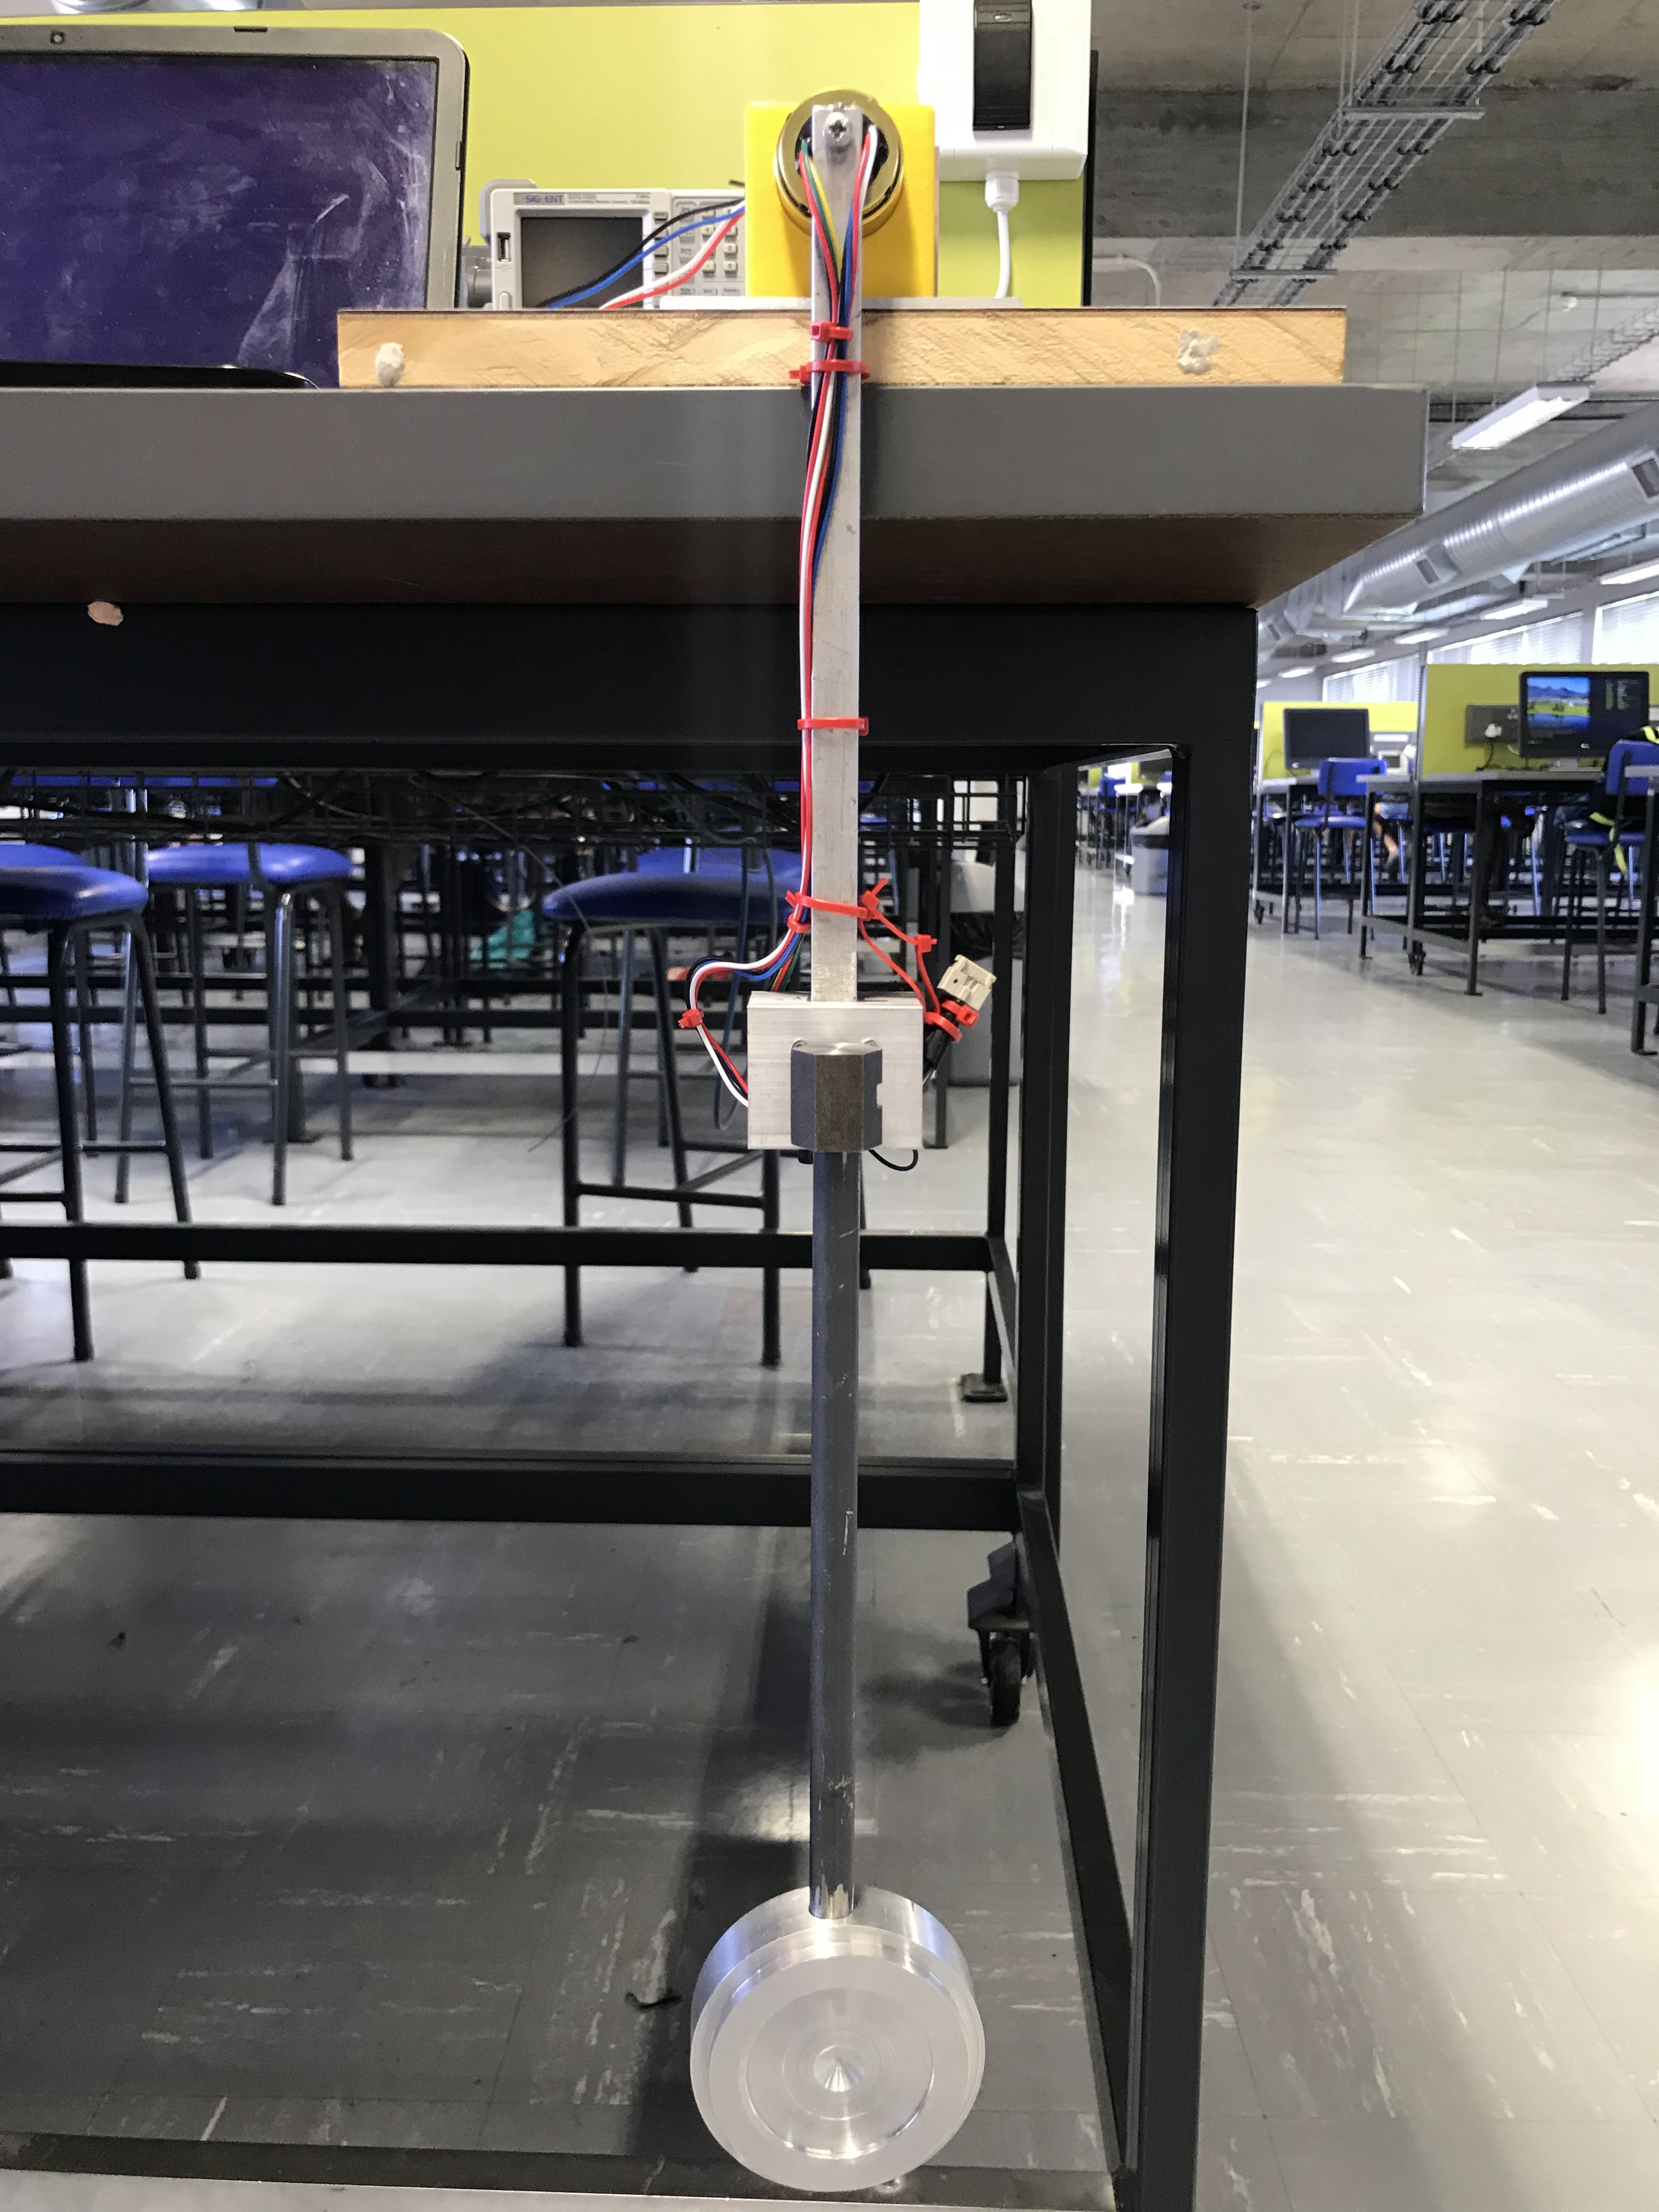
\includegraphics[width=\textwidth]{overview.jpg}};
    %microcontroller
    %\draw[green,ultra thick,rounded corners] (6.5,5) node[above]{ \textbf{MCU} };
    

    
    
    
    \draw[red,thick,->] (6,5) -- (8,5) node[right,white]{\contour{black}{Actuated Pendulum}};
    \draw[red,thick,->] (6,12) -- (8,12) node[right,white]{\contour{black}{Unactuated Pendulum}};
    \draw[red,thick,->] (6,8) -- (8,8) node[right,white]{\contour{black}{Torque Input \& Hinge}};	
    \draw[black,thick,->] (6.2,15) -- (8,15) node[right,white]{\contour{black}{Fixed Hinge}};	
    %XOR
    
    
\end{tikzpicture}
\end{document}